% Copyright 2022 Pierre S. Caboche. All rights reserved.

\renewcommand{\currentPart}{Running Solr}
\part{\currentPart}  \label{part - Running Solr}

In this part, we will learn how to run Solr, index documents, then run queries. \\

For ease of use:
\begin{itemize}
	\item Solr will be run as a Docker container
	\item documents to index will in the form of JSON files
	\item some scripts will be provided to launch the Docker container and index the JSON files
\end{itemize}

\texttt{sample\_song\_file.json}
\lstinputlisting{files/bsd-licensed/songs/sample_song_file.json}
\bigskip







\section{Getting starting with Solr}

In this section we will see the scripts used to start Solr, create the core, load the documents, etc. 

\subsection{Starting Solr} \label{starting-solr}

\texttt{mysolr.sh} \label{mysolr.sh}
\lstinputlisting[language=sh]{files/bsd-licensed/solr/mysolr.sh}
\bigskip


This script accepts one parameter (the action to take), which is one of the following: 

\begin{description}
	\item[start] \hfill (default)
	
	The \texttt{start} option will first try to detect if the Docker container already exists or not. If the container does not exist, it will try to create it (from the latest Docker image for Solr) and initialise it (including loading the songs data from JSON files). 
	
	If the Docker container already exits, the \texttt{start} option will start it. 
	
	It will then display the status of the Docker container (to confirm it is running). 
	
	\item[stop] \hfill
	
	The \texttt{stop} option will try to stop the Docker container.
	
	It will then display the status of the Docker container (to confirm it has stopped). 
	
	\item[rm] \hfill
	
	The \texttt{stop} option will try to stop and delete the Docker container.
	
	It will then try to display the status of the Docker container (this should not return anything).
	
	
	\item[enable\_mlt] \hfill
	
	This enables the \MLT\ (\emph{MLT}) feature, which is disabled by default (more details in \emph{section \longref{mlt}}). \\
	
	\texttt{mlt.fl} is a required parameter for the \MLT\ feature (i.e. the field we need to use to compare for similarities between documents). 
	We set it to have the value of: \texttt{lyrics\_txt\_ja}.\\
	This way we won't have to specify the \texttt{mlt.fl} parameter every time we want to use the \MLT\ feature.
	
\end{description}


\bigskip

It is also possible to modify the behaviour of the script by passing certain variables: \\

\begin{tabular}{l l l}
	\texttt{CONT\_SOLR} : & the Docker container name & (default: solr\_lyrics) \\
	\texttt{CORE} : & the core (collection) containing our songs & (default: songs\_jp) \\
	\texttt{HOST} : & the Solr host name & (default: localhost) \\
	\texttt{PORT} : & the Solr port & (default: 8983) \\
\end{tabular}


\bigskip


\subsection{Initialisation}  \label{initialisation}

The \texttt{\_init.sh} script will do the following:
\begin{enumerate}
	\item wait for the (containerised) Solr server to start
	\item create the Solr core to contain our songs
	\item load the data into our Solr core (\emph{see \ref{loading-songs}})
\end{enumerate}

\bigskip

Here is the script: \\

\texttt{\_init.sh}
\lstinputlisting[language=sh]{files/bsd-licensed/solr/_init.sh}
\bigskip




\bigskip

\subsection{Loading the songs} \label{loading-songs}

The loading of the songs data (from JSON files) is done by the script named

\texttt{load\_into\_solr.sh} \\


This script is automatically run during the initialisation (\emph{section \ref{initialisation}}), but you can also run it manually, to either add new songs or modify existing documents. \\


\subsubsection{Renaming fields} \label{renaming-fields}

Below is a sample JSON file containing a song information and lyrics: \\

\texttt{sample\_song\_file.json}
\lstinputlisting{files/bsd-licensed/songs/sample_song_file.json}
\bigskip




As explained in section \emph{\longref{dynamic-fields}}, we will rename some of the fields in our JSON files in order to use dynamic fields. This is easier than modifying the schema, and the field names will follow a convention that is easy to follow. \\

So the fields will be renamed as follows:

\begin{itemize}
	\item \texttt{title\_jp} $\rightarrow$ \texttt{title\_txt\_ja}
	\item \texttt{lyrics\_jp} $\rightarrow$ \texttt{lyrics\_txt\_ja}
	\item \texttt{band} $\rightarrow$ \texttt{band\_str}
	\item \texttt{lyrics\_by} $\rightarrow$ \texttt{lyrics\_by\_str}
	\item \texttt{music\_by} $\rightarrow$ \texttt{music\_by\_str}
\end{itemize}


As a reminder:

\begin{itemize}
	\item dynamic fields with the pattern ``\texttt{*\_txt\_ja} " are first tokenised and analysed using the Japanese text analyser (see \emph{section \longref{kuromoji}}): the analyser extracts all the lexemes and their positions from the text, and builds a \termsVector\ which is then used to index the field. 
	
	Searches on such fields is based on lexemes, distance between terms, and other criteria. This means that the search \emph{does not} need to be based on exact terms or phrases (but is based on relevance to the search terms).
	
	\item dynamic fields with the pattern ``\texttt{*\_str}" are of type \texttt{strings}. A \texttt{string} is not tokenised or analysed, which means that searches must be performed on the \emph{exact} terms.
	
	\texttt{strings} are used for short texts (with a hard limit of slightly less than 32K), and are useful to store things like: labels, categories, etc.
\end{itemize}

\bigskip

The script \texttt{\_alter\_json.sed} will rename the fields from the JSON files, so we can use the appropriate built-in dynamic fields instead (this is less effort than modifying the schema). \\

The \texttt{\_alter\_json.sed} script reads data from the standard input, renames the aforementioned fields, and writes the results in the standard output: \\

\texttt{\_alter\_json.sed}
\lstinputlisting[language=sh]{files/bsd-licensed/solr/_alter_json.sed}
\bigskip

The \texttt{\_alter\_json.sh} script is used when loading the documents into Solr. \\




\subsubsection{Loading the JSON files} \label{loading-JSON-files}


The \texttt{load\_into\_solr.sh} script does the following:

\begin{itemize}
	\item count the JSON files to import (using \texttt{find} and \texttt{wc -l} commands, so as to measure overall progress)
	
	\item list all the JSON files to import (with \texttt{find} command), and for each file:
	
	\begin{itemize}
		\item display a progress message
		\item read the JSON file, rename some fields to better fit our usage (see \emph{``\longref{renaming-fields}"})
		\item load the modified JSON document into Solr
	\end{itemize}
\end{itemize}

Below is the script: \\

\bigskip

\texttt{load\_into\_solr.sh}
\lstinputlisting{files/bsd-licensed/solr/load_into_solr.sh}
\bigskip


The first \texttt{find} is used to count the JSON files, to display the overall progress. \\

The second \texttt{find} is used to list and process the JSON files. \\

\texttt{find} outputs the files' path, one file per line. The file path may contain some spaces, special characters, single quotes (\texttt{'}), and double quotes (\texttt{"}). \\

In the file path, we will replace every single quotes it may contain (\texttt{'}) with (\texttt{'"'"'}). This will make it easier for us to generate a script in the next step. This is the role of the \texttt{sed} command. \\

The next step will generate a script for each file path (using \texttt{gawk}). This script will then be executed by \texttt{xargs}. \\

The script to be run by \texttt{xargs} contains several lines, therefore we cannot use the line feed character (\lstinline|\n|) as a separator, and will use the \lstinline|\0| character instead. As a consequence, we also invoke \texttt{xargs} with the \texttt{-0} option. \\

The AWK program, whose code is stored in the aptly named \texttt{AWK} variable (I didn't want to write a separate AWK script for this), does the following:
\begin{itemize}
	\item echoes a progress message (file number, total number of files, relative file path")
	
	\item reads the JSON file, rename fields (\emph{see \ref{renaming-fields}}) on the fly, and stores the result in the variable \texttt{DATA}
	
	\item sends the data to Solr, using \texttt{curl}
\end{itemize}

\bigskip

The script has been written in such a way that it is possible to load several files in parallel, by setting the \texttt{NB\_PROC} variable to a value higher than 1.

However, this does not change the loading time by much; at best it only saves a dozen seconds over the whole process. The indexing actually takes a bit of time (a few hundred milliseconds per document). \\




\newpage

\section{Using Solr} \label{using-solr}

As explained in section ``\longref{starting-solr}", we can start Solr with our \texttt{mysolr.sh} script (if necessary, this will download the Docker image for the latest version of Solr) : \\


\begin{lstlisting}[language=sh]
./mysolr.sh start
\end{lstlisting}

\bigskip

If everything worked fine, you will be able to connect to Solr on port 8983 (by default) :

\begin{center}
	\url{http://localhost:8983}
\end{center}



\begin{figure}[h]
	\centering
	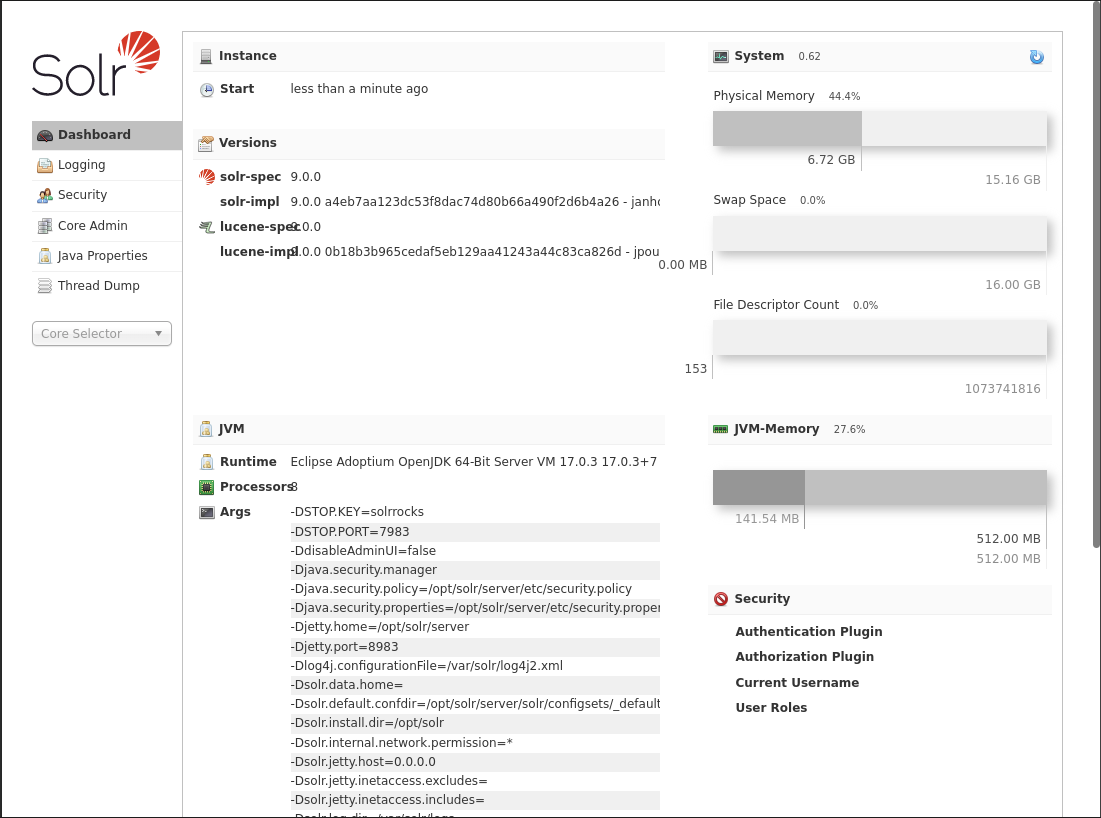
\includegraphics[width=0.75\linewidth]{files/images/solr-start-page}
	\caption{Solr start page}
	\label{fig:solr-start-page}
\end{figure}


In the ``Core Selector" drop-down, select the core we created (``songs\_jp") \\





From there, you can select ``Query" to start querying our dataset\dots (figure \ref{fig:solr-query}). \\

\newpage

\begin{figure}[h]
	\centering
	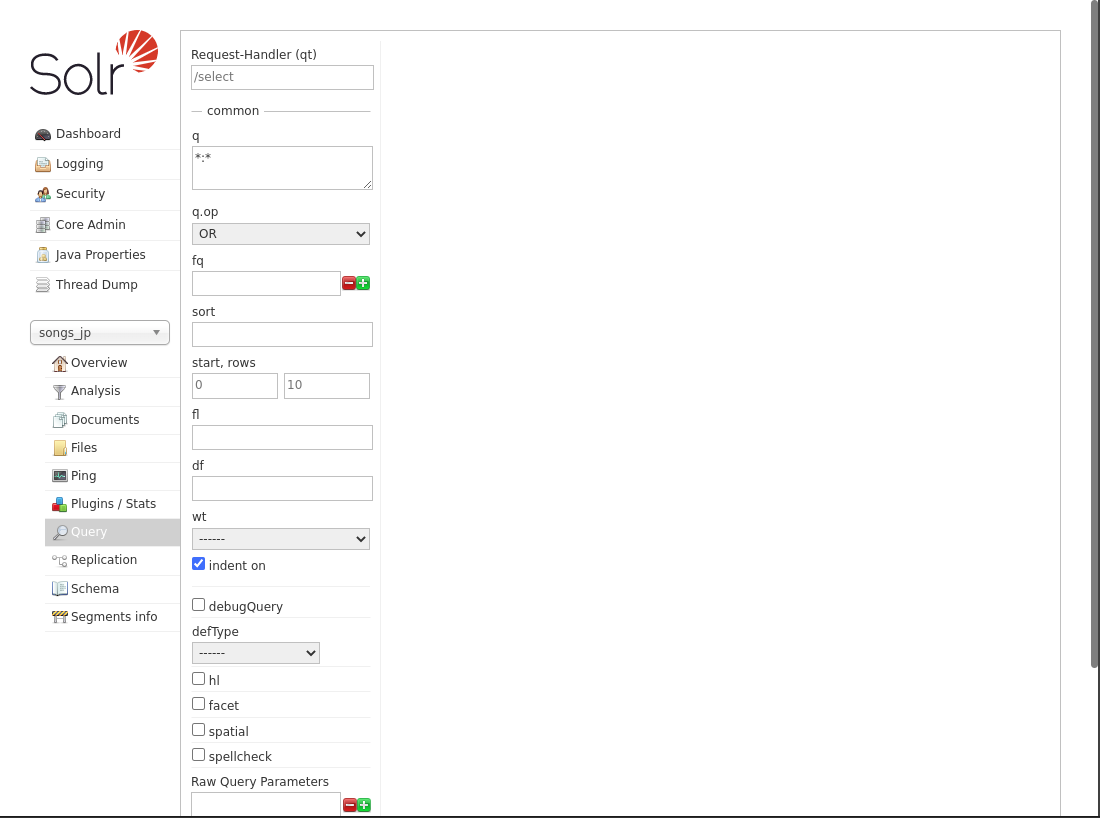
\includegraphics[width=0.75\linewidth]{files/images/solr-query}
	\caption{Solr query screen}
	\label{fig:solr-query}
\end{figure}

\bigskip

For our case study, we will mainly use the following fields from this screen:
\begin{itemize}
	\item \emph{fq}
	
	Stands for \emph{``filter query"}.
	
	We are going to use this field to filter out results (i.e. perform analysis only on a portion of our dataset).
	
	The default (\texttt{*:*}) does not filter anything.
	
	
	\item \emph{start, rows} \hfill default: \texttt{0,10}
	
	These are two positive integer values.
	
	They indicate which documents from the result-set to output: \texttt{start} (a.k.a. \emph{offset}), and number of \texttt{rows}.
	
	In our study, we are more interested in the result of the \faceting\ than the records themselves. 
	
	This means we will usually set both of these values to 0.
	
	\item \emph{facet}
	
	This is the field we are the most interested in.
	
	We will enable it most of the time.
	
	\begin{itemize}
		\item \emph{facet.field}
		
		This is the field on which to perform the \faceting.
		
		We will perform the \faceting\ on fields of either type \texttt{strings} (e.g. 
		
		\texttt{band\_str}), or indexed \texttt{text} (e.g. \texttt{lyrics\_txt\_ja})
		
		
		\item \emph{facet.mincount}  % \hfill default: \texttt{0}
			
		This field tells Solr to remove the \emph{facets} with a low document count. 
		
		For example, by setting \emph{facet.mincount} to \emph{1}, \emph{facets} with no documents will not appear.
		
		If this field is left empty, Solr will effectively use 0 as a default value.
		
		\item \emph{facet.limit}   \hfill default: \texttt{100}
		
		The maximum number of constraint counts (i.e. the number of facets for a field that are returned) that should be returned.
		
		A negative value means unlimited number of facets. 
		
		
	\end{itemize}
\end{itemize}


\bigskip
\bigskip

After filling up the fields, click on \emph{``Execute Query"} to display the results (figure~\ref{fig:solr-query-result}):

\begin{figure}[h]
	\centering
	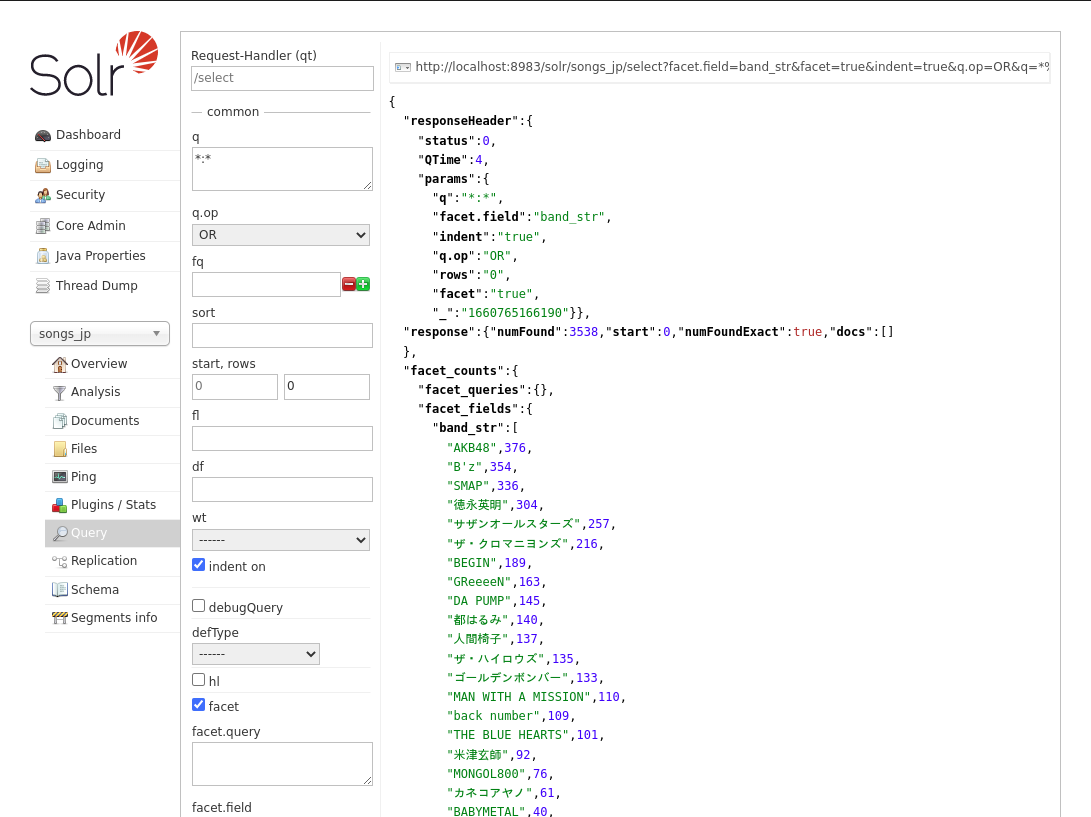
\includegraphics[width=0.75\linewidth]{files/images/solr-query-result}
	\caption{Solr query result}
	\label{fig:solr-query-result}
\end{figure}

\bigskip

Above the query result (in JSON), you can see a rather long URL. This shows the URL of web API for the current query (i.e. the kind of URL you will need to interact with Solr programmatically). \\

Clicking on the URL will display Solr's web API response, which is in JSON format (figure~\ref{fig:solr-web-api-result-json}):

\newpage

\begin{figure}[h]
	\centering
	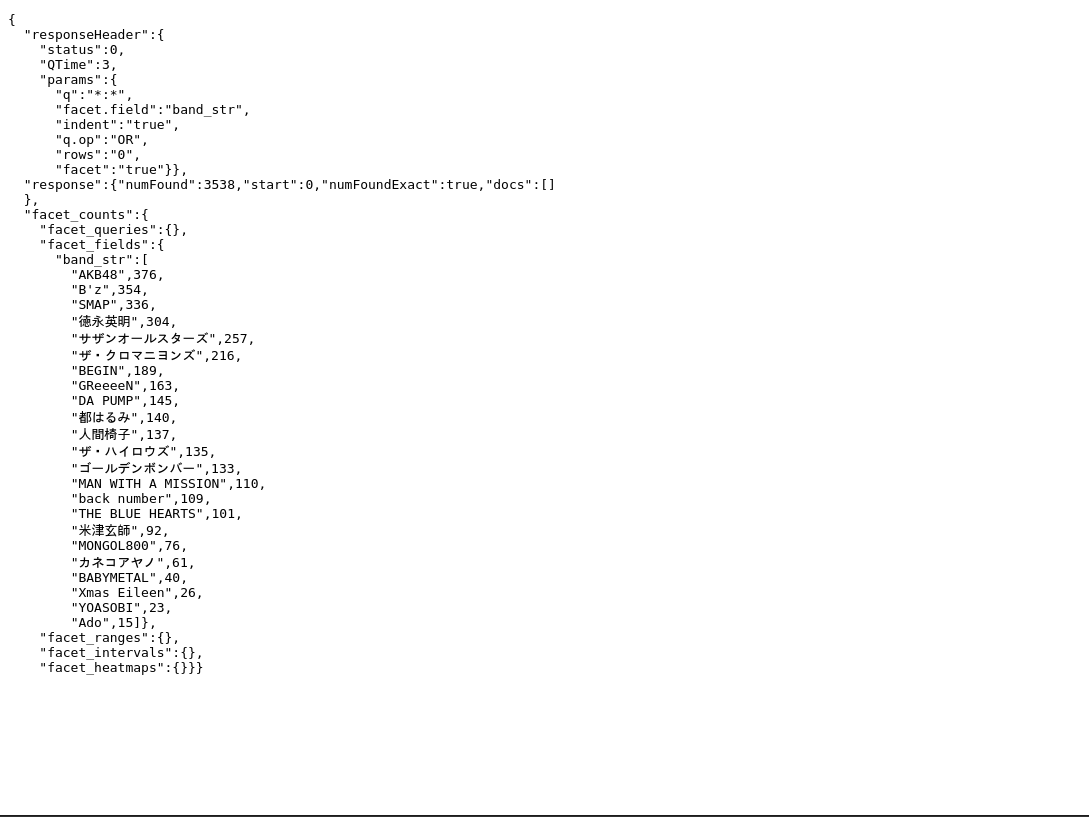
\includegraphics[width=0.75\linewidth]{files/images/solr-web-api-result}
	\caption{Solr - web API result}
	\label{fig:solr-web-api-result-json}
\end{figure}


\bigskip
\bigskip
\bigskip

Now that we are familiar with Solr, we all set to perform queries and analyse our dataset!

